%%%%%%%%%%%%%%%%%%%%%%%%%%%%%%%%%%%%%%%%%%%%%%%%%%%%%%%%%%%%%%%%%%%%%%%%%%%%
% AGUtmpl.tex: this template file is for articles formatted with LaTeX2e,
% Modified December 2018
%
% This template includes commands and instructions
% given in the order necessary to produce a final output that will
% satisfy AGU requirements.
%
% FOR FIGURES, DO NOT USE \psfrag
%
%%%%%%%%%%%%%%%%%%%%%%%%%%%%%%%%%%%%%%%%%%%%%%%%%%%%%%%%%%%%%%%%%%%%%%%%%%%%
%
% IMPORTANT NOTE:
%
% SUPPORTING INFORMATION DOCUMENTATION IS NOT COPYEDITED BEFORE PUBLICATION.
%
%
%
%%%%%%%%%%%%%%%%%%%%%%%%%%%%%%%%%%%%%%%%%%%%%%%%%%%%%%%%%%%%%%%%%%%%%%%%%%%%
%
% Step 1: Set the \documentclass
%
%
% PLEASE USE THE DRAFT OPTION TO SUBMIT YOUR PAPERS.
% The draft option produces double spaced output.
%
% Choose the journal abbreviation for the journal you are
% submitting to:

% jgrga JOURNAL OF GEOPHYSICAL RESEARCH (use for all of them)
% gbc   GLOBAL BIOCHEMICAL CYCLES
% grl   GEOPHYSICAL RESEARCH LETTERS
% pal   PALEOCEANOGRAPHY
% ras   RADIO SCIENCE
% rog   REVIEWS OF GEOPHYSICS
% tec   TECTONICS
% wrr   WATER RESOURCES RESEARCH
% gc    GEOCHEMISTRY, GEOPHYSICS, GEOSYSTEMS
% sw    SPACE WEATHER
% ms    JAMES
% ef    EARTH'S FUTURE
%
%
%
% (If you are submitting to a journal other than jgrga,
% substitute the initials of the journal for "jgrga" below.)

\documentclass[draft,jgrga]{agutexSI2019}

%%%%%%%%%%%%%%%%%%%%%%%%%%%%%%%%%%%%%%%%%%%%%%%%%%%%%%%%%%%%%%%%%%%%%%%%%
%
%  SUPPORTING INFORMATION TEMPLATE
%
%% ------------------------------------------------------------------------ %%
%
%
%Please use this template when formatting and submitting your Supporting Information.

%This template serves as both a “table of contents” for the supporting information for your article and as a summary of files.
%
%
%OVERVIEW
%
%Please note that all supporting information will be peer reviewed with your manuscript. It will not be copyedited if the paper is accepted.
%In general, the purpose of the supporting information is to enable authors to provide and archive auxiliary information such as data tables, method information, figures, video, or computer software, in digital formats so that other scientists can use it.
%The key criteria are that the data:
% 1. supplement the main scientific conclusions of the paper but are not essential to the conclusions (with the exception of
%    including %data so the experiment can be reproducible);
% 2. are likely to be usable or used by other scientists working in the field;
% 3. are described with sufficient precision that other scientists can understand them, and
% 4. are not exe files.
%
%USING THIS TEMPLATE
%
%***All references should be included in the reference list of the main paper so that they can be indexed, linked, and counted as citations.  The reference section does not count toward length limits.
%
%All Supporting text and figures should be included in this document. Insert supporting information content into each appropriate section of the template. To add additional captions, simply copy and paste each sample as needed.

%Tables may be included, but can also be uploaded separately, especially if they are larger than 1 page, or if necessary for retaining table formatting. Data sets, large tables, movie files, and audio files should be uploaded separately. Include their captions in this document and list the file name with the caption. You will be prompted to upload these files on the Upload Files tab during the submission process, using file type “Supporting Information (SI)”

%IMPORTANT NOTE ON FIGURES AND TABLES
% Placeholders for figures and tables appear after the \end{article} command, after references.
% DO NOT USE \psfrag or \subfigure commands.
%
 \usepackage{float}
 \usepackage{graphicx}
 \usepackage{subfigure} 
 \usepackage{lineno}
\linenumbers
 %\usepackage{subcaption}
% \usepackage{caption}
 %\usepackage{graphicx,caption,afterpage}
%
%  Uncomment the following command to allow illustrations to print
%   when using Draft:
 \setkeys{Gin}{draft=false}
%
% You may need to use one of these options for graphicx depending on the driver program you are using. 
%
% [xdvi], [dvipdf], [dvipsone], [dviwindo], [emtex], [dviwin],
% [pctexps],  [pctexwin],  [pctexhp],  [pctex32], [truetex], [tcidvi],
% [oztex], [textures]
%
%
%% ------------------------------------------------------------------------ %%
%
%  ENTER PREAMBLE
%
%% ------------------------------------------------------------------------ %%

% Author names in capital letters:
%\authorrunninghead{BALES ET AL.}

% Shorter version of title entered in capital letters:
%\titlerunninghead{SHORT TITLE}

%Corresponding author mailing address and e-mail address:
%\authoraddr{Corresponding author: A. B. Smith,
%Department of Hydrology and Water Resources, University of
%Arizona, Harshbarger Building 11, Tucson, AZ 85721, USA.
%(a.b.smith@hwr.arizona.edu)}

\begin{document}

%% ------------------------------------------------------------------------ %%
%
%  TITLE
%
%% ------------------------------------------------------------------------ %%

%\includegraphics{agu_pubart-white_reduced.eps}


\title{Poroelastic effects of the damage zone on fracture normal compliance and reflectivity}
%
% e.g., \title{Supporting Information for "Terrestrial ring current:
% Origin, formation, and decay $\alpha\beta\Gamma\Delta$"}
%
%DOI: 10.1002/%insert paper number here%

%% ------------------------------------------------------------------------ %%
%
%  AUTHORS AND AFFILIATIONS
%
%% ------------------------------------------------------------------------ %%


% List authors by first name or initial followed by last name and
% separated by commas. Use \affil{} to number affiliations, and
% \thanks{} for author notes.
% Additional author notes should be indicated with \thanks{} (for
% example, for current addresses).

% Example: \authors{A. B. Author\affil{1}\thanks{Current address, Antartica}, B. C. Author\affil{2,3}, and D. E.
% Author\affil{3,4}\thanks{Also funded by Monsanto.}}

\authors{ ...}


% \affiliation{1}{First Affiliation}
% \affiliation{2}{Second Affiliation}
% \affiliation{3}{Third Affiliation}
% \affiliation{4}{Fourth Affiliation}

\affiliation{=number=}{=Affiliation Address=}
%(repeat as many times as is necessary)


%% ------------------------------------------------------------------------ %%
%
%  BEGIN ARTICLE
%
%% ------------------------------------------------------------------------ %%

% The body of the article must start with a \begin{article} command
%
% \end{article} must follow the references section, before the figures
%  and tables.

\begin{article}

%% ------------------------------------------------------------------------ %%
%
Last changes 

\begin{itemize}
    \item  Figure \ref{fig:2} shows the sensitivity of various dimensionless rock and fluid properties to the ratio $Z_N^o/Z_N^u$ (equation \ref{eq1}).
    \item Figure \ref{fig:3}b shows the results for $|T_{PP}|$ as a function of DZ permeability.
    \item Figure \ref{fig:8} shows results for rock properties corresponding to shales.
    \item Figure \ref{fig:9} shows results for fluid properties corresponding to supercritical $CO_2$ saturating only the DZ and fracture. The elastic background is water saturated.
    \item Figure \ref{fig:10} was redone to reflect the aforementioned changes. This figure shows the ratio of absolute values of normally-incident P-wave reflectivity taken between the results of the poroelastic $|R_{PP}^p|$ and corresponding elastic $|R_{PP}^e|$.
    
    \item All figures related to the elastic-viscoelastic model were removed.
\end{itemize}

To  calculate the low and high frequency limits of compliance: $Z_N^o$ and $Z_N^u$, respectively, we use the formulae proposed by \cite{Rubino2015a}:
\begin{equation}\label{eq1}
    Z_N^u =  \frac{h}{H},\qquad
    Z_N^o = Z_N^u + \frac{2B(B-B_r)}{\frac{2B}{\alpha \,Z_N^d} + \frac{M_r(1-\alpha_r B_r)}{h_r}},
\end{equation}
where $Z_N^d$ is the drained fracture compliance, h refers to layer thickness, H and M are the undrained and drained plane-wave modulus, respectively, $\alpha$ is the Biot-Willis parameter and B is the Skemption coefficient. The subscript r refers to the damage zone (DZ) and no subscript refers to the poroelastic fracture. Equation \ref{eq1} is used to explain reflectivity changes as a consequence of changes of rock and fluid properties of the fracture and DZ.

% The following is a comment regarding Figure \ref{fig:10}b that compares poroelastic compliance $Z_N^p$ with the compliance derived from the elastic linear slip (LS) theory $Z_N^{LS}$. Probably not to be included in the paper. A different perspective regarding this discrepancy can be considered when the formula for the normal P-reflectivity  ($R_{PP}$) derived from the LS theory \cite{schoenberg1980elastic} is re-arranged as:

% $$  V_{P_r}= \frac{2 R_{PP}}{ i \rho_r \omega (1+R_{PP}) Z_N}, $$
% where $V_{P_r}$  and $\rho_r$ are the P-wave velocity and density for DZ, respectively, $i$ is the imaginary unit and $\omega$ is the angular frequency.
% We assume that $R_{PP}$ is constant and that $Z_N$ could be either $Z_N^p$ or $Z_N^{LS}$. Moreover according to Figure \ref{fig:9}b, $Z_N^p > Z_N^{LS}$. Then for $Z_N = Z_N^p$, the above equation predicts a lower $ V_{P_r}$ than for $Z_N = Z_N^{Ls}$. We have been assuming that $V_{P_r}$ is equal to the elastic undrained velocity, but  if we would like to use the normal compliance as predicted by poroelasticity then a lower velocity is required ... Below my additional thoughts regarding this.

% In Figure \ref{fig:11} we show that it is possible to obtain a frequency-dependent moduli $M_e(\omega)$ representing mechanically both the poroelastic fracture and associated poroelastic DZ layers. Furthermore, following \citeA{Rubino2015a} we show that it is also possible to obtain a viscoleastic fracture compliance $Z_N^v(\omega)$. Then, considering a viscoelastic effective medium context, could it be possible to obtain the corresponding moduli $M_r (\omega)$ for a DZ layer, given that we already have $M_e(\omega)$ and $Z_N^v(\omega)$?.  Could this provide a solution for the issue I raised in the above paragraph regarding $ V_{P_r}$?.
%
%% ------------------------------------------------------------------------ %%


%%%
%\noindent\textbf{Contents of this file}
%%%Remove or add items as needed%%%
\begin{enumerate}
% \item Text S1 to Sx
% \item Figures S1 to Sx
% \item Tables S1 to Sx

%if Tables are larger than 1 page, upload as separate excel file
\end{enumerate}

%\noindent\textbf{Additional Supporting Information (Files uploaded separately)}
\begin{enumerate}
% \item Captions for Datasets S1 to Sx
% \item Captions for large Tables S1 to Sx (if larger than 1 page, upload as separate excel file)
% \item Captions for Movies S1 to Sx
% \item Captions for Audio S1 to Sx
\end{enumerate}

%\noindent\textbf{Introduction}
%Type or paste your text here. The introduction gives a brief overview of the supporting information. You should include information %about as many of the following as possible (when appropriate):
% 1. a general overview of the kind of data files;
% 2. information about when and how the data were collected or created;
% 3. a general description of processing steps used;
% 4. any known imperfections or anomalies in the data.

%\clearpage

%Delete all unused file types below. Copy/paste for multiples of each file type as needed.

%\noindent\textbf{Text S1.}
%Type or paste text here. This should be additional explanatory text, such as: extended descriptions of results, full details of models, extended lists of acknowledgements etc.  It should not be additional discussion, analysis, interpretation or critique. It should not be an additional scientific experiment or paper.
%
%Repeat for any additional Supporting Text

%%Enter Data Set, Movie, and Audio captions here
%%EXAMPLE CAPTIONS

%\noindent\textbf{Data Set S1.} %Type or paste caption here.
%upload your dataset(s) to AGU's journal submission site and select "Supporting Information (SI)" as the file type. Following naming %convention: ds01.

%Repeat for any additional Supporting data sets'

%\noindent\textbf{Movie S1.} %Type or paste caption here.
%upload your movie(s) to AGU's journal submission site and select, "Supporting Information %(SI)" as the file type. Following naming convention: ms01.

%Repeat any additional Supporting movies

%\noindent\textbf{Audio S1.} %Type or paste caption here.
%upload your audio file(s) to AGU's journal submission site and select "Supporting Information %(SI)" as the file type. Following naming convention: auds01.


%Repeat for any additional Supporting audio files

%%% End of body of article:
%%%%%%%%%%%%%%%%%%%%%%%%%%%%%%%%%%%%%%%%%%%%%%%%%%%%%%%%%%%%%%%%
%
% Optional Notation section goes here
%
% Notation -- End each entry with a period.
% \begin{notation}
% Term & definition.\\
% Second term & second definition.\\
% \end{notation}
%%%%%%%%%%%%%%%%%%%%%%%%%%%%%%%%%%%%%%%%%%%%%%%%%%%%%%%%%%%%%%%%


%% ------------------------------------------------------------------------ %%
%%  REFERENCE LIST AND TEXT CITATIONS

%%%%%%%%%%%%%%%%%%%%%%%%%%%%%%%%%%%%%%%%%%%%%%%
% 
%
% \bibliography{<name of your .bib file>} do not specify file extension
%
% no need to specify bibliographystyle
%
% Note that ALL references in this supporting information file must also be referenced in the primary manuscript
%
%%%%%%%%%%%%%%%%%%%%%%%%%%%%%%%%%%%%%%%%%%%%%%%
% if you get an error about newblock being undefined, uncomment this line:
%\newcommand{\newblock}{}

 \bibliography{reference.bib } 




%Reference citation instructions and examples:
%
% Please use ONLY \cite and \citeA for reference citations.
% \cite for parenthetical references
% ...as shown in recent studies (Simpson et al., 2019)
% \citeA for in-text citations
% ...Simpson et al (2019) have shown...
% DO NOT use other cite commands (e.g., \citet, \citep, \citeyear, \nocite, \citealp, etc.).
%
%
%...as shown by \citeA{jskilby}.
%...as shown by \citeA{lewin76}, \citeA{carson86}, \citeA{bartoldy02}, and \citeA{rinaldi03}.
%...has been shown \cite<e.g.,>{jskilbye}.
%...has been shown \cite{lewin76,carson86,bartoldy02,rinaldi03}.
%...has been shown \cite{lewin76,carson86,bartoldy02,rinaldi03}.
%
% apacite uses < > for prenotes, not [ ]
% DO NOT use other cite commands (e.g., \citet, \citep, \citeyear, \nocite, \citealp, etc.).
%

%% ------------------------------------------------------------------------ %%
%
%  END ARTICLE
%
%% ------------------------------------------------------------------------ %%
\end{article}
\clearpage

% Copy/paste for multiples of each file type as needed.

% enter figures and tables below here: %%%%%%%
%

\begin{table}[!ht]
\begin{center}
  \begin{tabular}{ | l | c | c| }
    \hline
    Property & DZ & Fracture \\ \hline
    Grain bulk modulus $K_s$ ($GPa$) & 37 & 37 \\ 
    Grain density $\rho_s$ ($Kg/m^3$) & 2730 & 2730 \\
    Porosity $\phi$ & 0.015 & 0.8 \\
    Frame bulk modulus $K_m$ ($GPa$) & 33 & 0.004\\ 
    Frame shear modulus $\mu$ ($GPa$) & 29 & 0.002 \\
    Thickness $h$ ($m$) & 0.2 & 0.001\\ 
    Permeability $\kappa$ ($D$) & 0.1 & 100\\
    Tortuosity $S$ & 3 & 8\\
    Fluid density $\rho_f$ ($Kg/m^3$) & 1000 & 1000\\
    Fluid bulk modulus $K_f$ ($GPa$) & 2.25 & 2.25\\
    Fluid viscosity $\eta$ ($Pa.s$)& 0.001 & 0.001\\
    \hline
  \end{tabular}
  \caption{Reference values of the physical properties for the DZ, fracture and pore fluid. Furthermore the corresponding drained normal fracture compliance $Z_N^d $ and tangential fracture compliance $Z_t$ are 1.5e-10 m/Pa and 5e-10 m/Pa, respectively.}
  \label{table:1}
\end{center}
\end{table}

 \begin{figure}[!ht]
\centering
\subfigure[]{
        \centering
        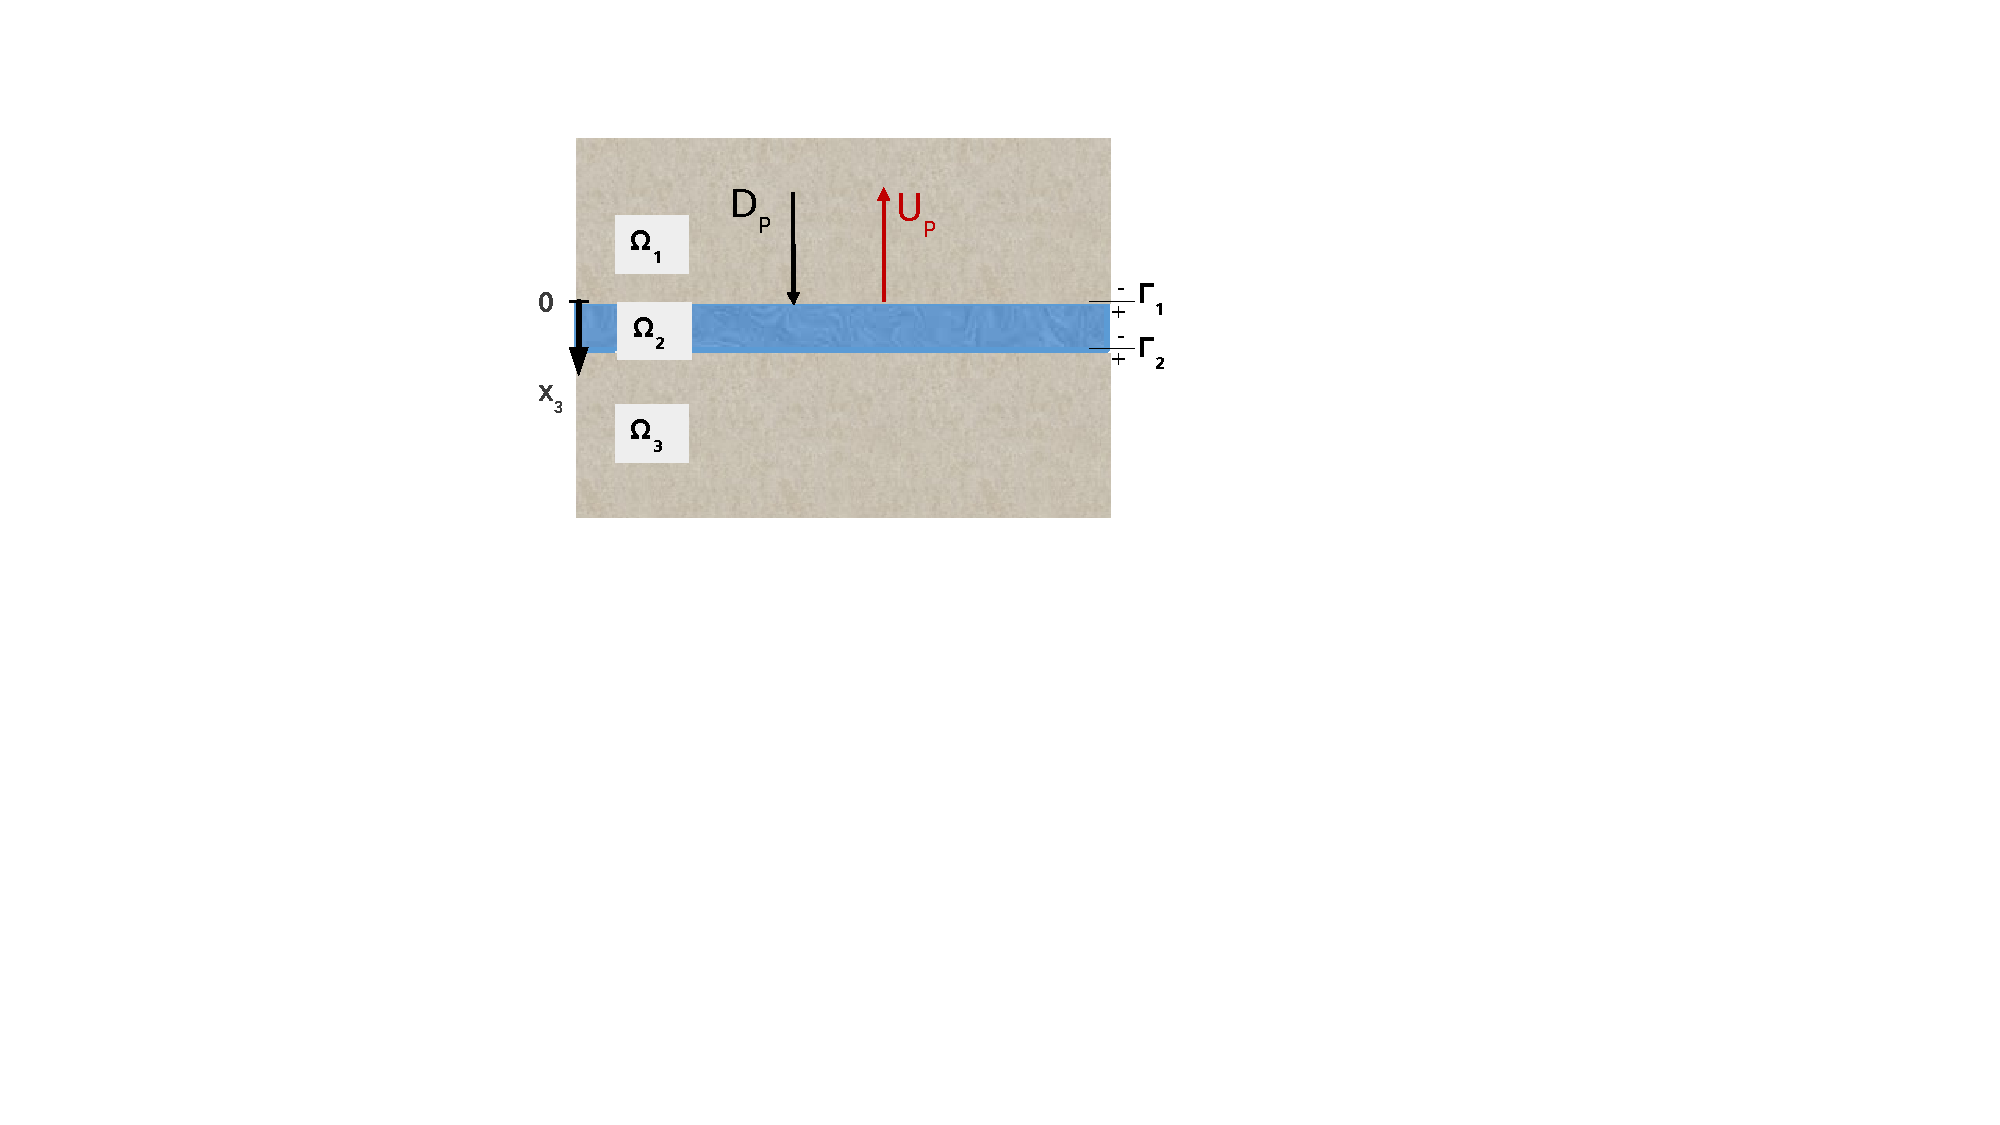
\includegraphics[width= 46mm, height=31mm]{./figures/elastic-model.pdf}
        %\label{}
        }
\subfigure[]{
        \centering
        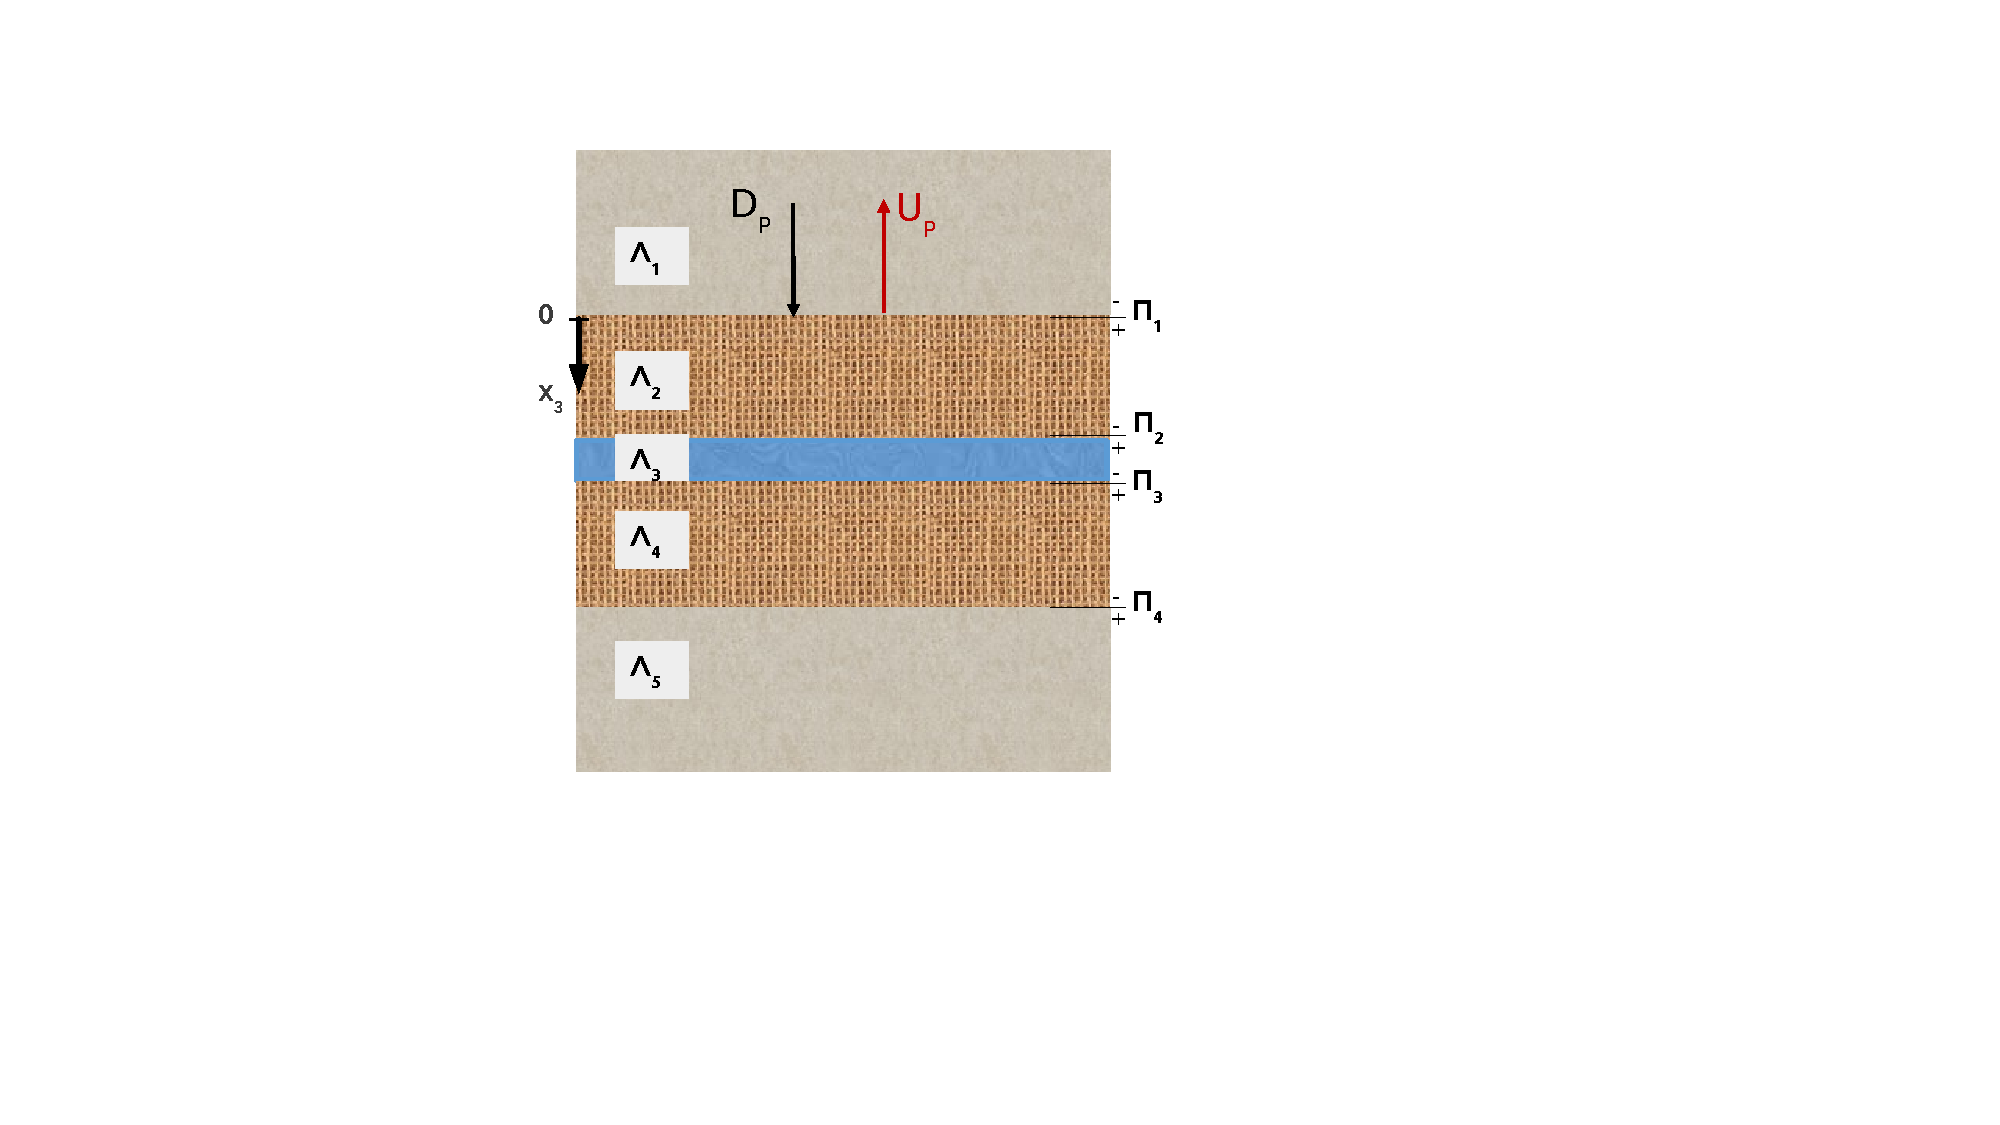
\includegraphics[width=46mm, height=45mm]{./figures/elastic-poro-model.pdf}
        %\label{}
        }
        
    
\caption{ a) Elastic model. b) Elastic-poroelastic model. $D_P$ and $U_P$ are the incident and reflected P-waves, respectively. }
\label{fig:1}
\end{figure}

 \begin{figure}[!ht]
\centering
        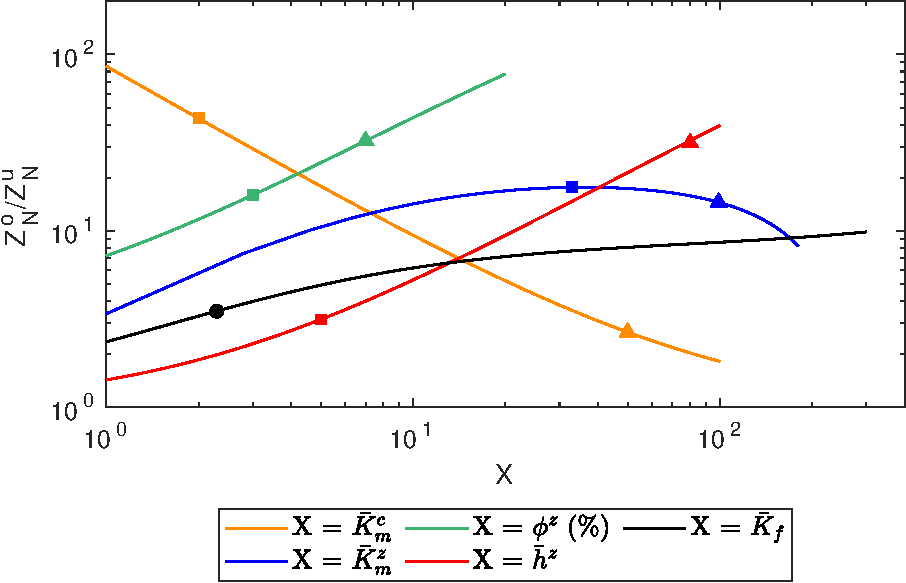
\includegraphics[width=100mm, height=60mm]{figures/zno_znu_sensitivity.pdf}
        %\label{}
\caption {Ratio of the low-frequency limit normal compliance $Z_N^o$ to the undrained normal compliance $Z_N^u$ as function of frequency of different dimensionless rock and fluid parameters $X$ of the fracture and DZ (equation \ref{eq1}). Varying parameters are: the drained plane wave-modulus of the fracture $H_d$, the drained plane wave-modulus of DZ $H_d^r$, the DZ porosity $\phi_r$, the DZ thickness $h_r$ and the fluid bulk modulus $K_f$. The corresponding reference values are: $H_d^o =0.67\, MPa$, $H_d^{ro} =9.8 \,GPa$, $h_{ro}=0.01\, m$ and $K_f^o= 10 \,MPa$}
\label{fig:2}
\end{figure}

 \begin{figure}[!ht]
\centering
  \subfigure[]{
        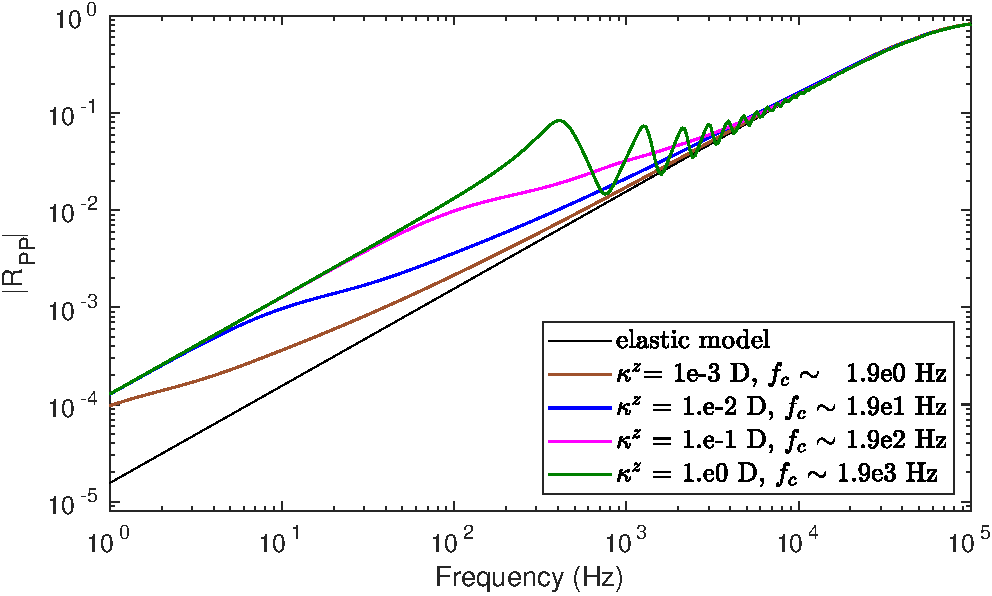
\includegraphics[width=80mm, height=50mm]{figures/elasporo_1mm_ksen_h20e-2.pdf}
        %\label{}
        }
        
          \subfigure[]{
        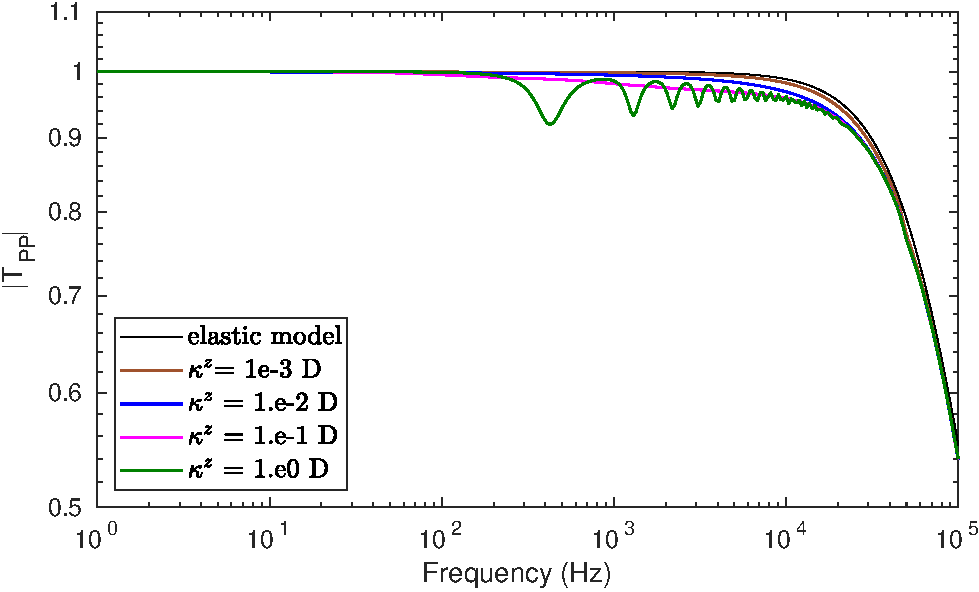
\includegraphics[width=80mm, height=50mm]{figures/TPPelasporo_1mm_ksen_h20e-2.pdf}
        %\label{}
        }
\caption {(a) Absolute value of normal P-wave reflectivity $|R_{PP}|$ as a function of frequency for different DZ permeabilities $\kappa_r$. (b)  Absolute value of normal P-wave transmission coefficient  $|R_{PP}|$ as a function of frequency for different DZ permeabilities $\kappa_r$.}
\label{fig:3}
\end{figure}


\begin{figure}[hp]
\centering
     \subfigure[]{
       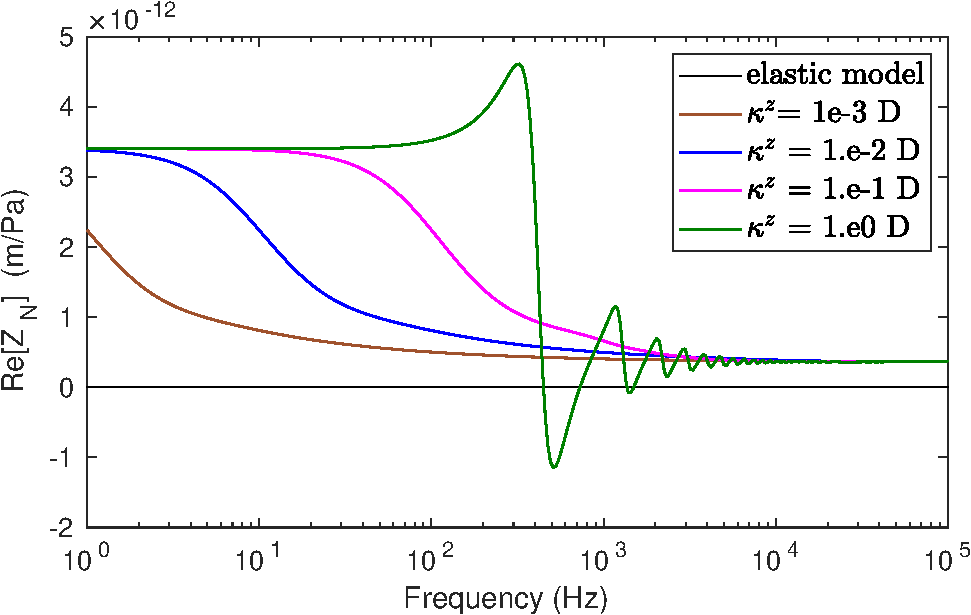
\includegraphics[width=73mm, height=43 mm]{figures/elasporo_1mm_znsen_h20e-2.pdf}
        %\label{}
        }
        \subfigure[]{
        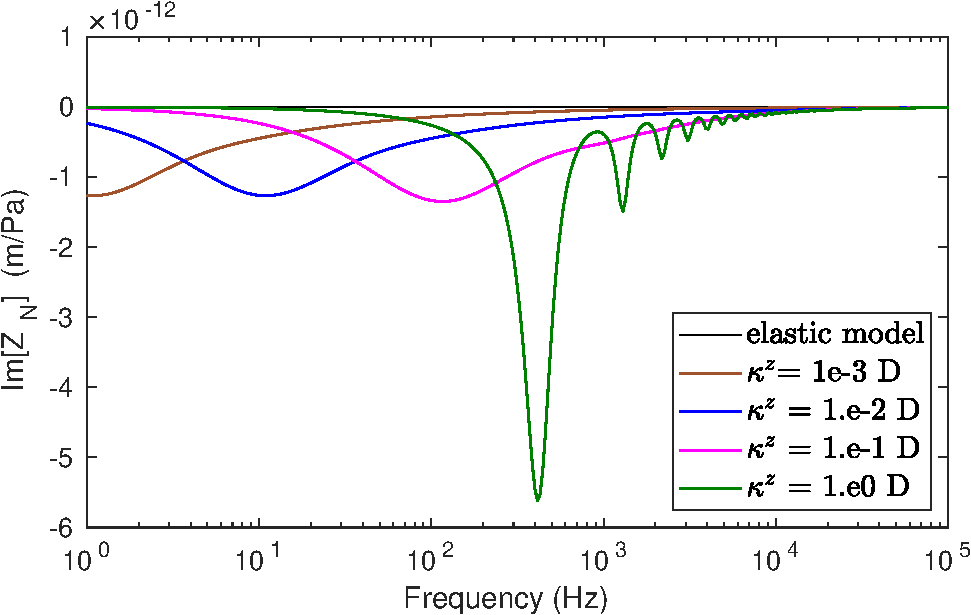
\includegraphics[width=73mm, height=43mm]{figures/elasporo_1mm_iznsen_h20e-2.pdf}
        %\label{}
        }
\caption {(a) Real and (b) imaginary parts of normal fracture compliance $Z_N$ as a function of frequency for different DZ permeabilities $\kappa_r$ and the reference rock and fluid properties from table \ref{table:1}. For the high frequency limit, the compliance $Z_N^u$ is 8.6e-13 m/Pa and for the low frequency limit, the compliance $Z_N^o$ is 3.4e-12 m/Pa. Moreover, The ratio $Z_N^o/Z_N^u$ is 9.45. } 
\label{fig:4}
\end{figure}

\begin{figure}[hp]
\centering
        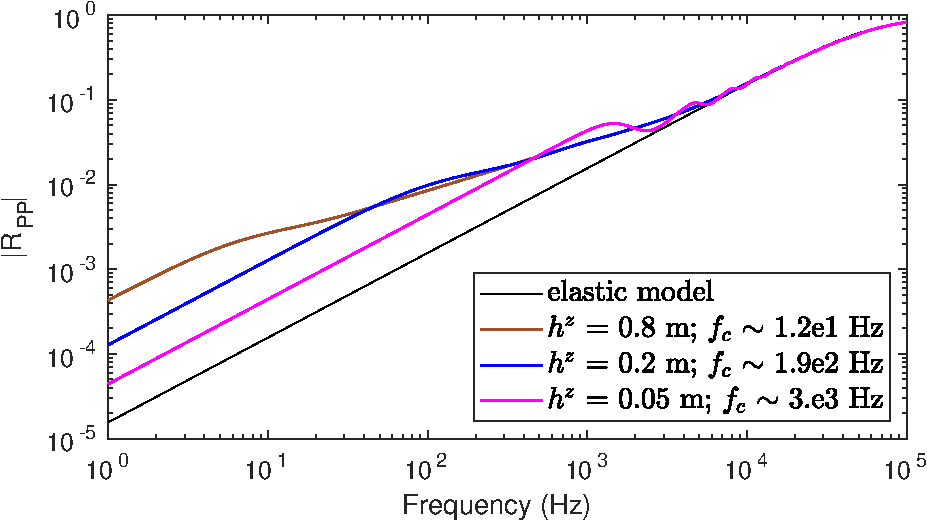
\includegraphics[width=80mm, height=50mm]{figures/elasporo_1mm_hsen_k1e-1d.pdf}
        %\label{}

\caption {Absolute value of normal P-wave reflectivity $|R_{PP}|$ as a function of frequency for different DZ thicknesses $h_r$.}
\label{fig:5}
\end{figure}

\begin{figure}[hp]
\centering
     \subfigure[]{
       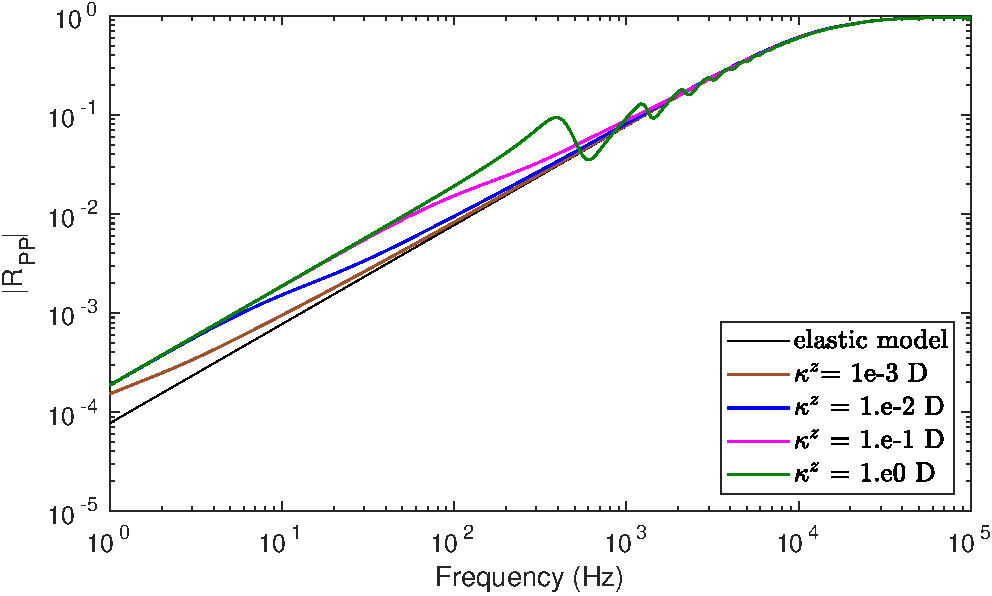
\includegraphics[width=73mm, height=43 mm]{figures/elasporo_5mm_ksen_h20e-2.pdf}
        %\label{}
        }
        \subfigure[]{
        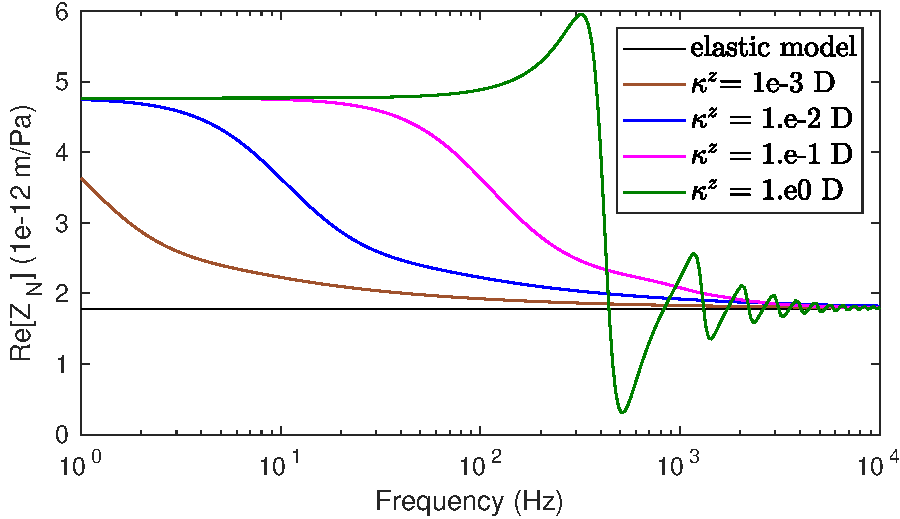
\includegraphics[width=73mm, height=43mm]{figures/elasporo_5mm_znsen_h20e-2.pdf}
        %\label{}
        }
\caption {Plots for a fracture with 5mm of thickness and same $Z_N^d$ as the reference fracture. Corresponding values for $K_m$ and $\mu$ are 0.02 GPa and 0.01 GPa, respectively. (a) Absolute value of normal P-wave reflectivity $|R_{PP}|$ as a function of frequency for different DZ permeabilities $\kappa_r$.(b) Real part of normal fracture compliance $Z_N$ as a function of frequency for different DZ permeabilities $\kappa_r$. Notice the higher values of reflectivity compared to those from the reference model (Figure \ref{fig:3}a). However, there is a correspondingly smaller increase of reflectivity for the poroelastic models with respect to the elastic reference. Regarding normal fracture compliance, notice the higher $Z_N^o =$ 4.77e-12 m/Pa and $Z_N^u =$ 1.78e-12 m/Pa compared to the reference model (Figure \ref{fig:4}a), but lower $Z_N^o/Z_N^u= $ 2.67.
}
\label{fig:6}
\end{figure}


\begin{figure}[hp]
\centering
     \subfigure[]{
       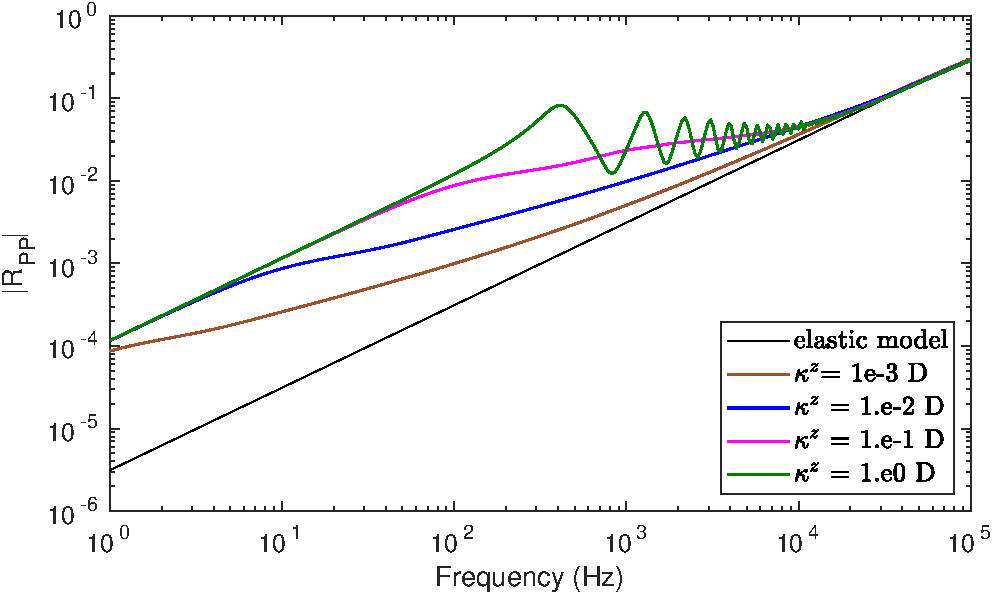
\includegraphics[width=73mm, height=43 mm]{figures/elasporo_02mm_ksen_h20e-2.pdf}
        %\label{}
        }
        \subfigure[]{
        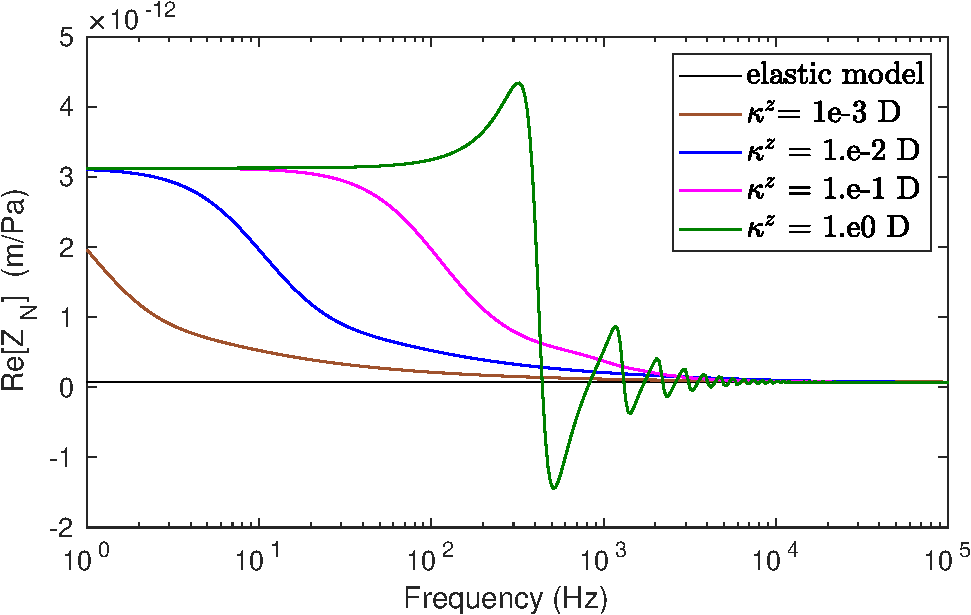
\includegraphics[width=73mm, height=43mm]{figures/elasporo_02mm_znsen_h20e-2.pdf}
        %\label{}
        }
\caption {Plots for a fracture with 0.2 mm of thickness and same $Z_N^d$ as the reference fracture. Corresponding values for $K_m$ and $\mu$ are 8e-4 GPa and 4e-4 GPa, respectively. (a) Absolute value of normal P-wave reflectivity $|R_{PP}|$ as a function of frequency for different DZ permeabilities $\kappa_r$.(b) Real part of normal fracture compliance $Z_N$ as a function of frequency for different DZ permeabilities $\kappa_r$. Notice the lower values of reflectivity compared to those from the reference model (Figure \ref{fig:3}a), However there is  a correspondingly greater increase of reflectivity for the poroelastic cases with respect to the elastic reference, close to two order-magnitude. Regarding normal fracture compliance, notice the lower $Z_N^o =$ 3.13e-12 m/Pa and $Z_N^u =$ 7.22e-14 m/Pa compared to the reference model (Figure \ref{fig:4}a), but higher $Z_N^o/Z_N^u= $ 43.35.}
\label{fig:7}
\end{figure}

\begin{figure}[hp]
\centering
     \subfigure[]{
       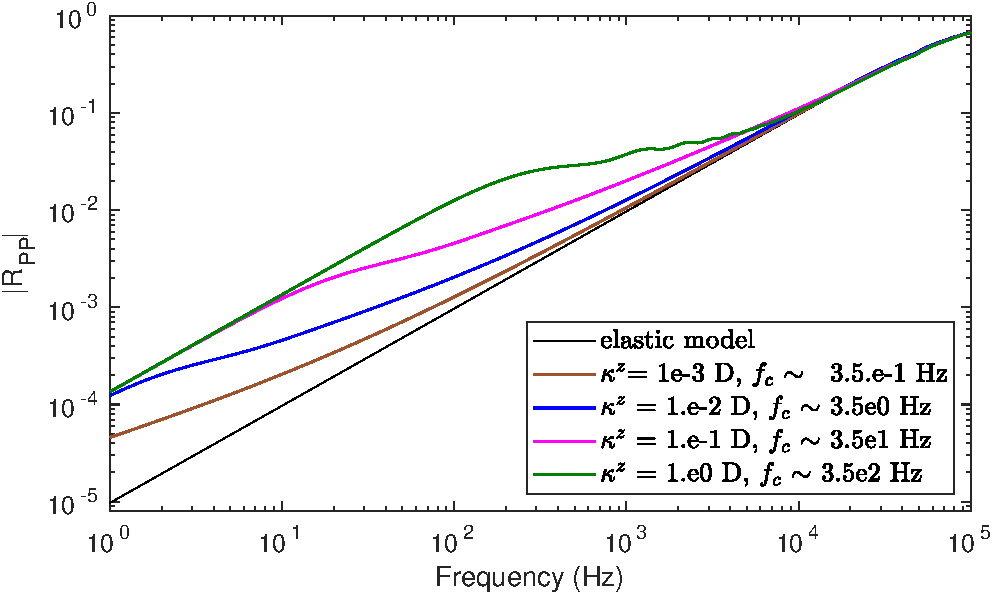
\includegraphics[width=73mm, height=43 mm]{figures/elasporo_1mm_shalev_ksen_h20e-2.pdf}
        %\label{}
        }
        \subfigure[]{
        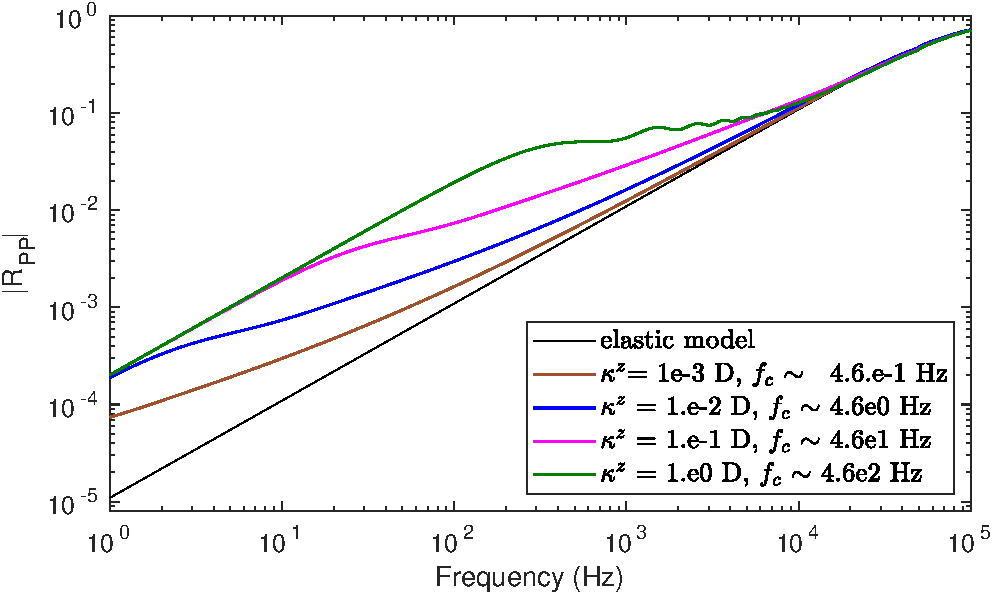
\includegraphics[width=73mm, height=43mm]{figures/elasporo_1mm_shaleh_ksen_h20e-2.pdf}
        %\label{}
        }
\caption {Plots considering  rock properties of a shale formation for DZ and the elastic background. Values  and $\phi$ and $\rho_s$ are 0.05 and 2650 $Kg/m^3$, respectively. We consider that shales exhibits a vertical transverse isotropy (VTI).   (a) Absolute value of normal P-wave reflectivity $|R_{PP}|$ as a function of frequency for different DZ permeabilities $\kappa_r$. We assume that the VTI line of symmetry is parallel to $\hat x_3$ (Figure \ref{fig:2}, eg. fracture parallel to the shale bedding plane) . We also assume that $K_m$ and $\mu$ have values of  12.5 GPa and 5 GPa, respectively, for both the DZ and elastic background.
(b) Real part of normal fracture compliance $Z_N$ as a function of frequency for different DZ permeabilities $\kappa_r$.  We assume that the VTI line of symmetry is perpendicualat to $\hat x_3$ (Figure \ref{fig:2}, eg. fracture perpendicular to the shale bedding plane). We also assume that $K_m$ and $\mu$ have values of  14.4 GPa and 9.6 GPa, respectively, for both the DZ and elastic background.}

% Notice that the reflectivity values for the elastic case is similar to those obtained with the reference model (Figure \ref{fig:2}) but the increase of reflectivity for the poroelastic cases with respect to the elastic reference is greater, more than one order-magnitude.}

\label{fig:8}
\end{figure}

\begin{figure}[hp]
\centering
     \subfigure[]{
       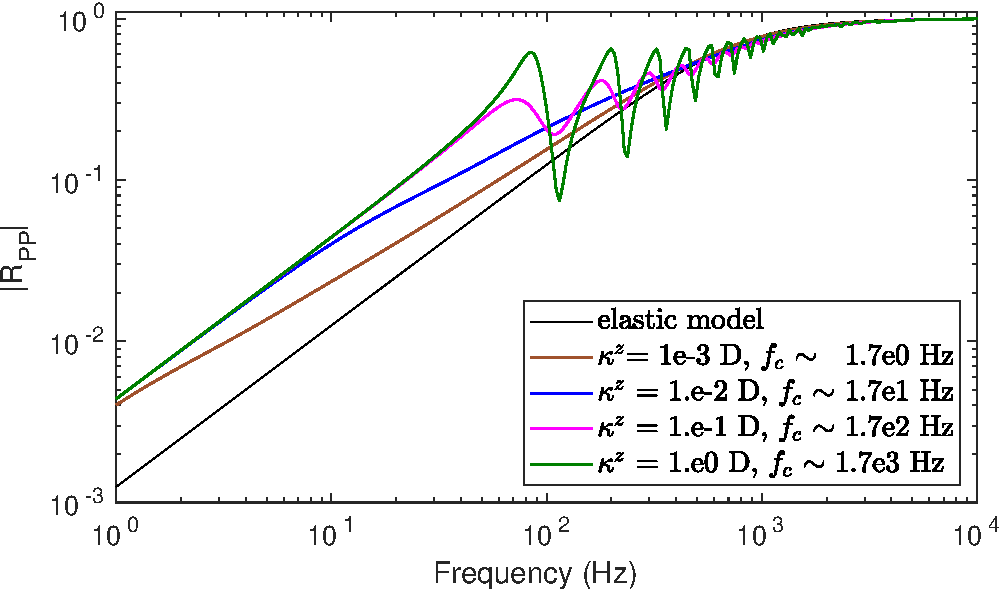
\includegraphics[width=70mm, height=43 mm]{figures/elasporo_1mm_co2fdz_ksen_h20e-2.pdf}
        %\label{}
        }
        \subfigure[]{
        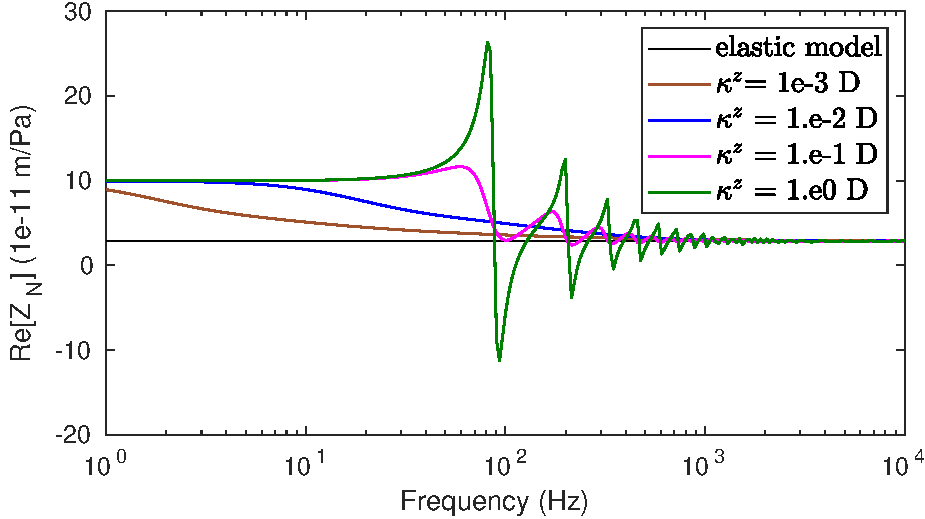
\includegraphics[width=73mm, height=43mm]{figures/elasporo_1mm_co2fdz_znsen_h20e-2.pdf}
        %\label{}
        }
\caption {Plots considering a more compressible and less viscous pore fluid such as $CO_2$ in supercritical state saturating both the DZ and fracture pores. The elastic background is considered to be water saturated. Values for $K_f$, $\rho_f$ and $\eta$ are 0.0229 GPa, 693 $kg/m^3$ and 1.56e-4 poise, respectively. (a) Absolute value of normal P-wave reflectivity $|R_{PP}|$ as a function of frequency for different DZ permeabilities $\kappa_r$.(b) Real part of normal fracture compliance $Z_N$ as a function of frequency for different DZ permeabilities $\kappa_r$. Notice that the reflectivity values for the elastic case are greater to those obtained with the reference model (Figure \ref{fig:3}a) but the increase of reflectivity for the poroelastic cases is lower, less than one order-magnitude. Moreover also notice the earlier onset of scattering effects for $K_r$ values of 1.e0 D and 1e-1 D. Biot's frequency ($f_b$) for these DZ permeabilities are 1.8e1 Hz and 1.8e2 Hz, respectively, as a consequence of this relative low $f_b$ values, propagating slow P-waves create scattering events.}
% Regarding normal fracture compliance, notice that  $Z_N^o =$ 9.96e-11 m/Pa and $Z_N^u =$ 2.83e-11 m/Pa are greater than for the reference model(Figure \ref{fig:3}a) but $Z_N^o/Z_N^u= $ 3.51 is lower.}
\label{fig:9}
\end{figure}

 \begin{figure}[!ht]
\centering
        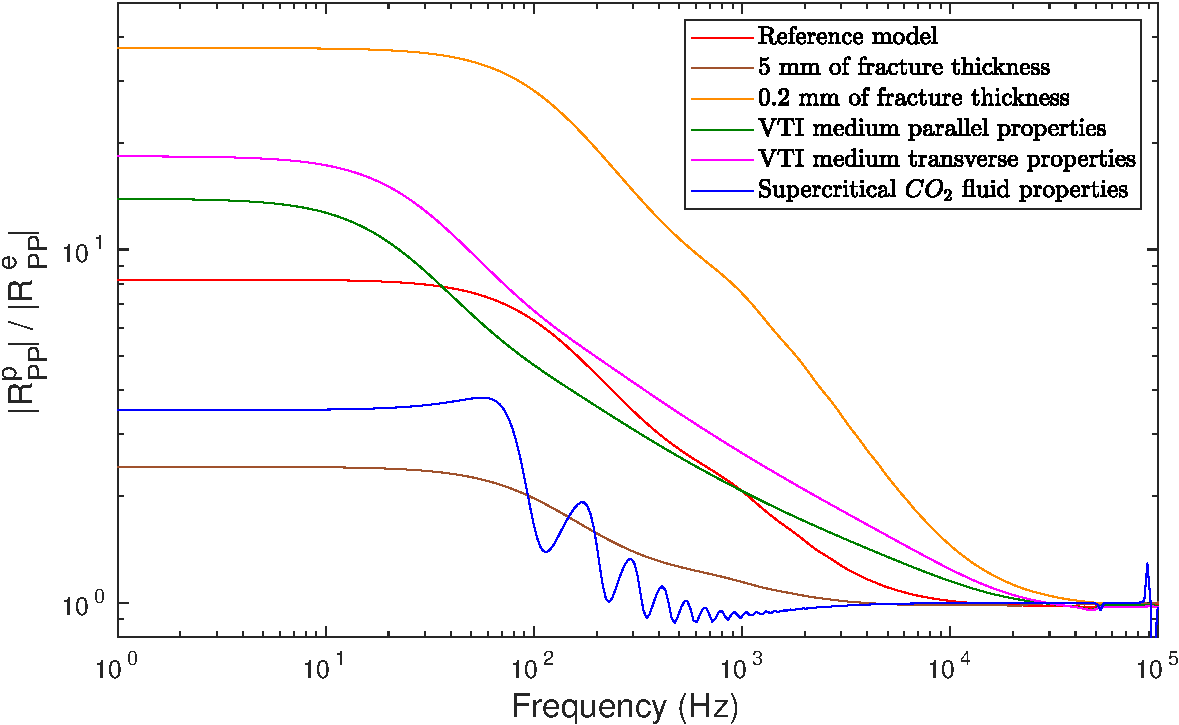
\includegraphics[width=110mm, height=70mm]{figures/ratioRT_elasporo_elas.pdf}
        %\label{}
\caption {Ratio of absolute values of normally-incident P-wave reflectivity taken between the poroelastic ($|R_{PP}^p|$) and corresponding elastic ($|R_{PP}^e|$) model results. The reference model corresponds to that with rock and fluid properties taken from table \ref{table:1}.}
\label{fig:10}
\end{figure}

\begin{figure}[hp]
\centering
     \subfigure[]{
       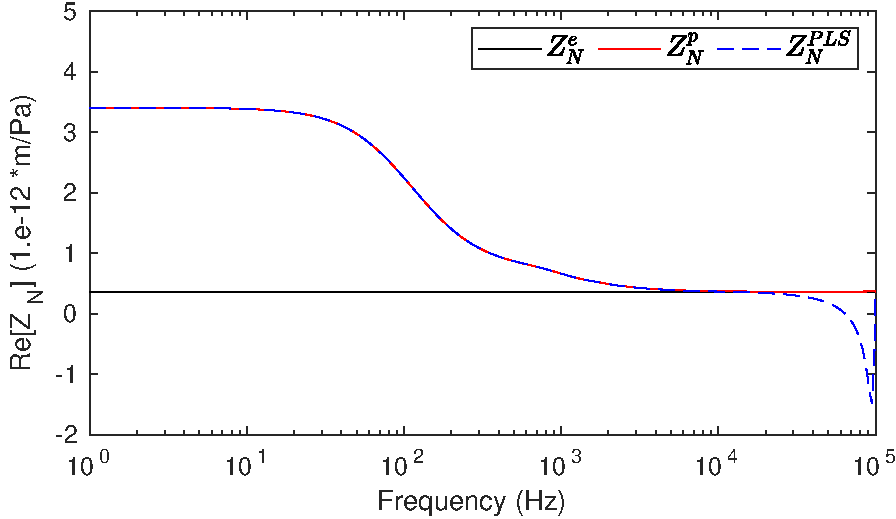
\includegraphics[width=73mm, height=43 mm]{figures/Zn_PLS_compare_1mm_1e-1d.pdf}
        %\label{}
        }
        \subfigure[]{
        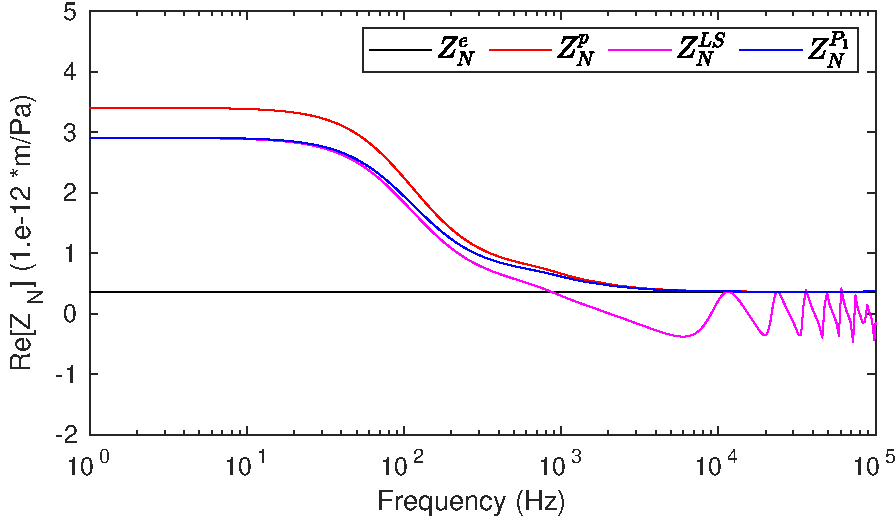
\includegraphics[width=73mm, height=43mm]{figures/Zn_compare_1mm_1e-1d.pdf}
        %\label{}
        }
\caption {Comparison of different estimates of fracture compliance $Z_N$ for the reference properties according table \ref{table:1}. Superscripts e and p refer to the elastic and poroelastic compliance, respectively, calculated following \citeA{schoenberg1980elastic}. We compare $Z_N^e$ and $Z_N^p$ against (a) $Z_N^{PLS} = Z_N^d \, t_{\hat x_3}^d /t_{\hat x_3}$ and  b) $Z_N^{LS}$  and $Z_N^{P_1}$. The superscript PLS denotes the poroelastic linear slip method, $t_{\hat x_3}^d$ and $t_{\hat x_3}$ refer to the normally applied traction on the drained rock frame and on the fluid-filled porous rock, respectively, at the fracture interface. The formula to obtain $Z_N^{PLS}$ is an extension of the displacement jump boundary condition formulated by \citeA{Nakagawa2007}. The extra term is  $t_{\hat x_3}$. $Z_N^{LS}$ is obtained by using the poroelastic reflectivity results and applying the elastic Linear slip (LS) theory \cite{schoenberg1980elastic} for a normally incident P-wave. $Z_N^{P_1}$ is obtained following the modification to the LS theory proposed by \citeA{Barbosa2017}. }
\label{fig:11}
\end{figure}

% \begin{figure}[hp]
% \centering
%      \subfigure[]{
%       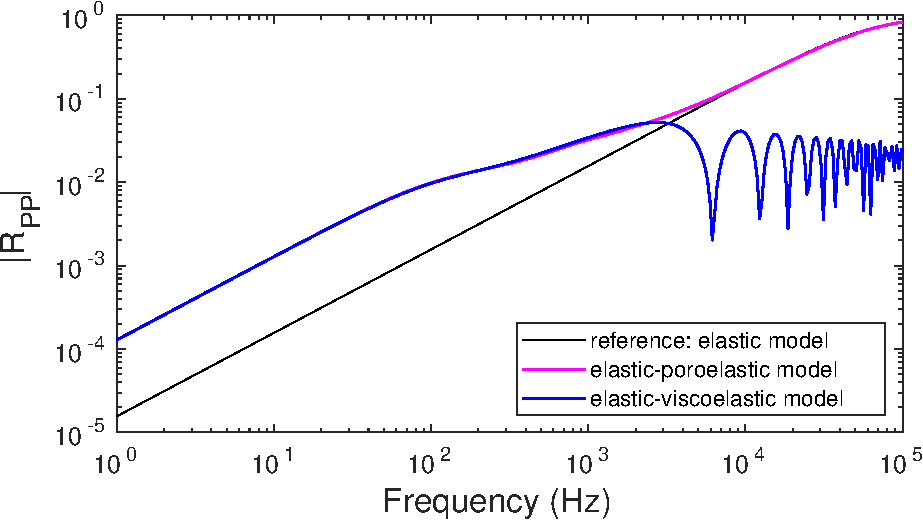
\includegraphics[width=73mm, height=43 mm]{figures/rt_elasvisco_1mm_1e-1d.pdf}
%         %\label{}
%         }
%         \subfigure[]{
%         \includegraphics[width=73mm, height=43mm]{figures/Zn_elasvisco_compare_1mm_1e-1d.pdf}
%         %\label{}
%         }
% \caption {(a) Absolute value of reflectivity  $|R_{PP}|$  and (b) real part of normal fracture compliance $Z_N$ as a function of frequency for various models. Superscripts e, p and v denote elastic, poroelastic and viscoelastic media, respectively. Values of rock and fluid properties are taken from table 1.}
% \label{fig:11}
% \end{figure}

%
% EXAMPLE FIGURES
% ---------------
% If you get an error about an unknown bounding box, try specifying the width and height of the figure with the natwidth and natheight options.
% \begin{figure}
%\setfigurenum{S1} %%You can change number for each figure if you want, not required. "S" prepended automatically.
% \noindent\includegraphics[natwidth=800px,natheight=600px]{samplefigure.eps}
%\caption{caption}
%\label{epsfiguresample}
%\end{figure}
%
%
% Giving latex a width will help it to scale the figure properly. A simple trick is to use \textwidth. Try this if large figures run off the side of the page.
% \begin{figure}
% \noindent\includegraphics[width=\textwidth]{anothersample.png}
%\caption{caption}
%\label{pngfiguresample}
%\end{figure}
%
%
%\begin{figure}
%\noindent\includegraphics[width=\textwidth]{athirdsample.pdf}
%\caption{A pdf test figure}
%\label{pdffiguresample}
%\end{figure}
%
% PDFLatex does not seem to be able to process EPS figures. You may want to try the epstopdf package.
%
%
% ---------------
% EXAMPLE TABLE
%
%\begin{table}
%\settablenum{S1} %%Change number for each table
%\caption{Time of the Transition Between Phase 1 and Phase 2\tablenotemark{a}}
%\centering
%\begin{tabular}{l c}
%\hline
% Run  & Time (min)  \\
%\hline
%  $l1$  & 260   \\
%  $l2$  & 300   \\
%  $l3$  & 340   \\
%  $h1$  & 270   \\
%  $h2$  & 250   \\
%  $h3$  & 380   \\
%  $r1$  & 370   \\
%  $r2$  & 390   \\
%\hline
%\end{tabular}
%\tablenotetext{a}{Footnote text here.}
%\end{table}
% ---------------
%
% EXAMPLE LARGE TABLE (UPLOADED SEPARATELY)
%\begin{table}
%\settablenum{S1} %%Change number for each table
%\caption{Time of the Transition Between Phase 1 and Phase 2\tablenotemark{a}}
%\end{table}


\end{document}

%%%%%%%%%%%%%%%%%%%%%%%%%%%%%%%%%%%%%%%%%%%%%%%%%%%%%%%%%%%%%%%

More Information and Advice:

%% ------------------------------------------------------------------------ %%
%
%  SECTION HEADS
%
%% ------------------------------------------------------------------------ %%

% Capitalize the first letter of each word (except for
% prepositions, conjunctions, and articles that are
% three or fewer letters).

% AGU follows standard outline style; therefore, there cannot be a section 1 without
% a section 2, or a section 2.3.1 without a section 2.3.2.
% Please make sure your section numbers are balanced.
% ---------------
% Level 1 head
%
% Use the \section{} command to identify level 1 heads;
% type the appropriate head wording between the curly
% brackets, as shown below.
%
%An example:
%\section{Level 1 Head: Introduction}
%
% ---------------
% Level 2 head
%
% Use the \subsection{} command to identify level 2 heads.
%An example:
%\subsection{Level 2 Head}
%
% ---------------
% Level 3 head
%
% Use the \subsubsection{} command to identify level 3 heads
%An example:
%\subsubsection{Level 3 Head}
%
%---------------
% Level 4 head
%
% Use the \subsubsubsection{} command to identify level 3 heads
% An example:
%\subsubsubsection{Level 4 Head} An example.
%
%% ------------------------------------------------------------------------ %%
%
%  IN-TEXT LISTS
%
%% ------------------------------------------------------------------------ %%
%
% Do not use bulleted lists; enumerated lists are okay.
% \begin{enumerate}
% \item
% \item
% \item
% \end{enumerate}
%
%% ------------------------------------------------------------------------ %%
%
%  EQUATIONS
%
%% ------------------------------------------------------------------------ %%

% Single-line equations are centered.
% Equation arrays will appear left-aligned.

Math coded inside display math mode \[ ...\]
 will not be numbered, e.g.,:
 \[ x^2=y^2 + z^2\]

 Math coded inside \begin{equation} and \end{equation} will
 be automatically numbered, e.g.,:
 \begin{equation}
 x^2=y^2 + z^2
 \end{equation}

% IF YOU HAVE MULTI-LINE EQUATIONS, PLEASE
% BREAK THE EQUATIONS INTO TWO OR MORE LINES
% OF SINGLE COLUMN WIDTH (20 pc, 8.3 cm)
% using double backslashes (\\).

% To create multiline equations, use the
% \begin{eqnarray} and \end{eqnarray} environment
% as demonstrated below.
\begin{eqnarray}
  x_{1} & = & (x - x_{0}) \cos \Theta \nonumber \\
        && + (y - y_{0}) \sin \Theta  \nonumber \\
  y_{1} & = & -(x - x_{0}) \sin \Theta \nonumber \\
        && + (y - y_{0}) \cos \Theta.
\end{eqnarray}

%If you don't want an equation number, use the star form:
%\begin{eqnarray*}...\end{eqnarray*}

% Break each line at a sign of operation
% (+, -, etc.) if possible, with the sign of operation
% on the new line.

% Indent second and subsequent lines to align with
% the first character following the equal sign on the
% first line.

% Use an \hspace{} command to insert horizontal space
% into your equation if necessary. Place an appropriate
% unit of measure between the curly braces, e.g.
% \hspace{1in}; you may have to experiment to achieve
% the correct amount of space.


%% ------------------------------------------------------------------------ %%
%
%  EQUATION NUMBERING: COUNTER
%
%% ------------------------------------------------------------------------ %%

% You may change equation numbering by resetting
% the equation counter or by explicitly numbering
% an equation.

% To explicitly number an equation, type \eqnum{}
% (with the desired number between the brackets)
% after the \begin{equation} or \begin{eqnarray}
% command.  The \eqnum{} command will affect only
% the equation it appears with; LaTeX will number
% any equations appearing later in the manuscript
% according to the equation counter.
%

% If you have a multiline equation that needs only
% one equation number, use a \nonumber command in
% front of the double backslashes (\\) as shown in
% the multiline equation above.

%% ------------------------------------------------------------------------ %%
%
%  SIDEWAYS FIGURE AND TABLE EXAMPLES
%
%% ------------------------------------------------------------------------ %%
%
% For tables and figures, add \usepackage{rotating} to the paper and add the rotating.sty file to the folder.
% AGU prefers the use of {sidewaystable} over {landscapetable} as it causes fewer problems.
%
% \begin{sidewaysfigure}
% \includegraphics[width=20pc]{samplefigure.eps}
% \caption{caption here}
% \label{label_here}
% \end{sidewaysfigure}
%
%
%
% \begin{sidewaystable}
% \caption{}
% \begin{tabular}
% Table layout here.
% \end{tabular}
% \end{sidewaystable}
%
%

